\chapter{Simulation data and Test Environment}
\label{ch:dataAndEnv}

This chapter introduces the input data and test environments.

\section{Raw data for training}
Details of selected data is introduced in Chapter~\ref{ch:market}, the date range is varied in different test, but is behind year 2009 as some data prior to the start date is hard to be collected. \\

The input data types are introduced in Chapter~\ref{ch:market}.\\

The stocks used here are those listed in HSI, there are 50 stocks in total. CK PROPERTY (1113.HK) is deleted as it is a really new stock (start from 2015-06-03). I replace it with HKT Trust and HKT Limited (6823.HK). Brief introduction information of some of those stocks can be found in Appendix~\ref{append:stock_info}.\\


\section{Testing Environment}
\label{sec:environment}
The model of physical computer is Dell Inspiron Ins14VD-4516, details about the hardware information is showed in table~\ref{tb:hardwareConf}, software are listed in table~\ref{tb:softwareList}
\begin{table}[h]
	\centering
	\begin{tabular}{|l|l|}
		\hline
		\textbf{Name} & \textbf{Details} \\ \hline
		CPU & Intel Core i5 4200U \\ \hline
		Memory & DDR3L 1600MHz 8GB(4GBx2) \\ \hline
		Hard disk & 500GB 5400 rpm \\ \hline
	\end{tabular}
	\caption{Hardware information}
	\label{tb:hardwareConf}
\end{table}

\begin{table}[h]
	\centering
	\begin{tabular}{|l|l|}
		\hline
		\textbf{Name} & \textbf{Details} \\ \hline
		OS & Ubuntu (Host version: 16.04, Guest version: 14.04) \\ \hline
		Virtualbox & Version 5.0.20 r106931 \\ \hline
		Python & 2.7.6 \\ \hline
		Apache Spark & 1.6.1 \\ \hline
		Hadoop & 2.6.0 \\ \hline
	\end{tabular}r
	\caption{Primary Software information}
	\label{tb:softwareList}
\end{table}
The cluster is formed by three virtual machines (as figure~\ref{fg:clustur}). "Master" is NameNode for HDFS, and Master, HistoryServer for Spark. The other two virtual machines work as DataNode (for HDFS) and worker (for Spark). Every computer has 40GB hard disk, 2GB memory and 1 virtual CPU core.
\begin{figure}[h]
	\centering
	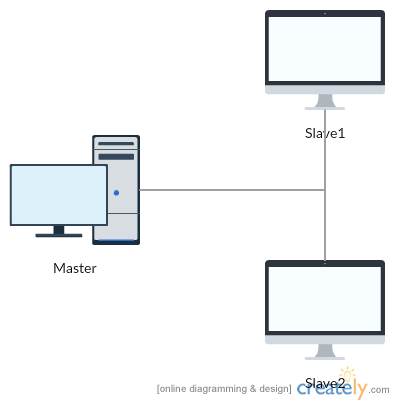
\includegraphics[width=0.6\textwidth]{ClusterStructure}
	\caption{Network Structure of the cluster}
	\label{fg:clustur}
\end{figure}
